\documentclass[letterpaper,12pt]{scrartcl}
\usepackage{epsfig,latexsym,amsmath,amssymb,epic,eepic,psfrag,subfigure,float,euscript,array}
\usepackage[latin1]{inputenc}
\usepackage[margin=24mm]{geometry}
\usepackage{enumitem}
\usepackage{tikz,pgf,pgfplots}
\usepgfplotslibrary{fillbetween}
\usetikzlibrary{decorations, arrows, patterns}

\usepackage[amssymb]{SIunits}

\usepackage{array}
\newcolumntype{L}{>{\[}l<{\]}} % math-mode version of "l" column type

\newenvironment{exercise}[1][Problem]{\begin{trivlist} \item[\hskip
    \labelsep {\stepcounter{exerctr}\bfseries #1
      \arabic{exerctr}}]}{\end{trivlist}\vspace{10mm}}

\newcounter{exerctr}
\newcounter{abcctr}[exerctr]

\newcommand{\abc}{\noindent\vspace{1mm}\\ {\bf
    \stepcounter{abcctr}(\alph{abcctr})\ }}
\newcommand{\bbm}{\begin{bmatrix}}
\newcommand{\ebm}{\end{bmatrix}}
\newcommand{\point}[1]{\hfill {\bf (#1p)}\\ \vspace{-5mm}}
\newcommand{\ctrb}{\EuScript{S}}
\newcommand{\Lap}{\mathcal{L}}
\newcommand{\obsv}{\EuScript{O}}
\newcommand{\realdel}{\text{Re}}
\newcommand{\imagdel}{\text{Im}}
\newcommand{\bC}{\mathbb{C}}
\newcommand{\bR}{\mathbb{R}}
\newcommand{\bmpv}{\begin{minipage}[t]}
\newcommand{\bmps}{\begin{minipage}[t]{45mm}}
\newcommand{\bmpm}{\begin{minipage}[t]{90mm}}
\newcommand{\bmpl}{\begin{minipage}[t]{\textwidth}}
\newcommand{\emp}{\end{minipage}}
\newcommand{\mexp}[1]{\ensuremath{\mathrm{e}^{#1}}}
\newcommand*{\laplaceinv}[1]{\ensuremath{\mathcal{L}^{-1} \left\{#1\right\}}}
\newcommand*{\ztrf}[1]{\ensuremath{\mathcal{Z} \left\{#1\right\}}}
\newcommand*{\shift}{\ensuremath{\operatorname{q}}}
\newcommand*{\diff}{\ensuremath{\operatorname{p}}}


\newcommand{\AxisRotator}[1][rotate=0]{%
    \tikz [x=0.2cm,y=0.60cm,line width=.1ex,-stealth,#1] \draw (0,0) arc (-150:150:1 and 1);%
}

\addtolength{\topmargin}{-8mm}
%\textheight 22.5cm
%\oddsidemargin 1.3cm
%\evensidemargin 1.3cm

\makeatletter
\newcommand*{\rom}[1]{\expandafter\@slowromancap\romannumeral #1@}
\makeatother

\newcommand*\circled[1]{\tikz[baseline=(char.base)]{
            \node[shape=circle,draw,inner sep=2pt] (char) {#1};}}


\title{Computerized Control Final exam (24\%)}
\author{Kjartan Halvorsen}
\date{}

\begin{document}

\maketitle


\begin{description}
\item[Time] May 4 16:10-18.10
\item[Place] 5105
\item[Permitted aids] The single colored page with your own notes, table of Laplace transforms, calculator
\end{description}

All answers should be readable and well motivated (if nothing else is written). Solutions/motivations should be written on the provided spaces in this exam. Use the last page if more space is needed.

\begin{center}
{\Large Good luck!} \\
\end{center}

\noindent
\fbox{
\bmpl
{\bf Matricula and name:}\\
\vspace*{14mm}
\emp}


%\clearpage

%-----------------------------------------------------------------

\subsection*{ABS brake system}
ABS (Anti-Blocking System) brakes are common on modern cars and motorcycles. Such braking systems will prevent the wheel from blocking when braking hard, reducing the distance needed to stop the vehicle and giving the driver the posibility to steer while braking.  
%The friction between a blocked wheel and the ground is less than the friction between a rolling wheel and ground, so an ABS brake will reduce the braking distance. Moreover, a blocked front wheel will not steer, since the friction force will be independent on the orientation of the wheel. Hence there are two important safety advantages with ABS brakes: The braking distance is shortened and the driver can steer while braking hard. 

Assume a wheel with radius $R$ on a vehicle travelling with the speed $V$. If the wheel is rolling freely (no brake torque or motor torque acting) the angular velocity of the wheel is \(\omega_v = \frac{V}{R}\). When braking, the wheel will slip, meaning its angular velocity will be less than \(\omega_v\). The \emph{wheel slip ratio} is defined as \(\lambda = \frac{\omega_v - \omega}{\omega_v}\), where \(\omega\) is the actual angular velocity of the wheel. The friction coefficient between wheel and surface is highly dependent on the wheel slip as shown in figure \ref{fig:muslip}. An ABS system will try to maintain a certain slip ratio \(\lambda=\lambda_{optimal}\) (around 0.1 -- 0.2) that gives the maximum friction.
\begin{figure}[!h]
\begin{center}
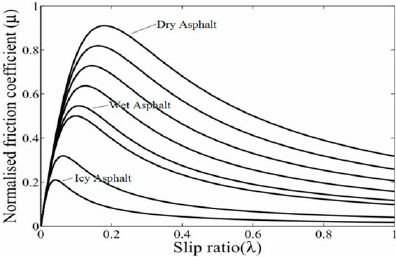
\includegraphics[width=0.4\linewidth]{typical-friction.png}
\caption{Dependency of friction coefficient \(\mu\) on the wheel slip. {\footnotesize From Pedro et al ``Direct adaptive neural control of antilock braking systems incorporated with passive suspension dynamics''  Journal of mechanical science and technology, 2013}}
\label{fig:muslip}
\end{center}
\end{figure}

The dynamics of the wheel is illustrated in figure \ref{fig:wheeldynamics}. The braking torque is produced by a hydraulic system pressing braking pistons against a metal disk. The friction force from the ground depends on the friction coefficient $\mu$ and the normal force $F_z$. 
\begin{figure}[!h]
\begin{center}
  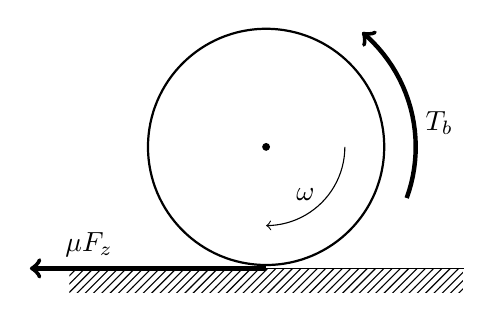
\begin{tikzpicture}
    \tikzstyle{ground}=[fill,pattern=north east lines,draw=none,minimum width=5cm,minimum height=0.3cm]
    
    \node[ground] (asfalt) {};
    \node[coordinate] (ax) at (0, 1.7) {};
    \draw (asfalt.north west) -- (asfalt.north east);
    \node[circle, draw, thick, minimum height=3cm] at (ax) {};
    \node[circle, fill, inner sep=0pt,minimum height=1mm] at (ax) {};
    \draw [->,black,domain=0:-90] plot ({cos(\x)}, {1.7+sin(\x)});
    \node at (0.5, 1.1) {$\omega$};
    \draw[->, ultra thick] (asfalt.north) -- node[above, near end] {$\mu F_z$} ++(-3,0);
    \draw [->,ultra thick, black,domain=-20:50] plot ({1.9*cos(\x)}, {1.7+1.9*sin(\x)});
    \node at (2.2, 2.0) {$T_b$};
  \end{tikzpicture}
  %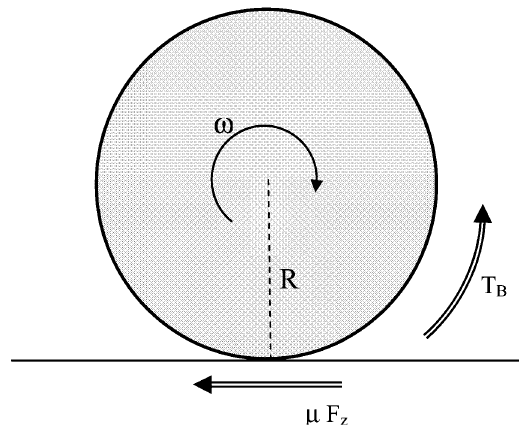
\includegraphics[width=0.3\linewidth]{wheel-rolling.png}
\caption{Forces acting on the wheel.}
\label{fig:wheeldynamics}
\end{center}
\end{figure}

A simplified and linearized model of the open-loop system is shown in figure \ref{fig:openloopblock}.
\begin{figure}[!h]
\begin{center}
  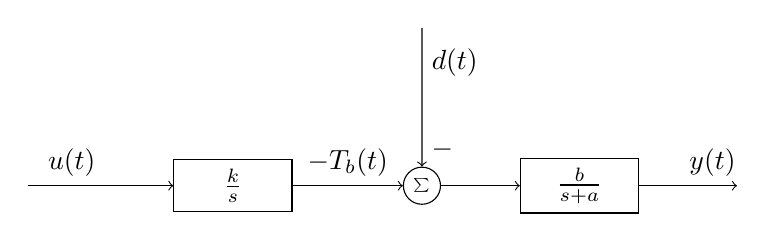
\begin{tikzpicture}[scale = 0.8, node distance=22mm, block/.style={rectangle, draw, minimum width=15mm}, sumnode/.style={circle, draw, inner sep=2pt}]
    
    \node[coordinate] (input) {};
     \node[block, right of=input, node distance=26mm] (int) {$\frac{k}{s}$};
     \node[sumnode, right of=int, node distance=24mm] (sumdist) {\tiny $\sum$};
     \node[block, right of=sumdist, node distance=20mm] (wheel) {$\frac{b}{s+a}$};
     \node[coordinate, right of=wheel, node distance=20mm] (output) {};
     \node[coordinate, above of=sumdist, node distance=20mm] (dist) {};

     \draw[->] (input) -- node[above, pos=0.3] {$u(t)$} (int);
     \draw[->] (int) -- node[above] {$-T_b(t)$} (sumdist);
     \draw[->] (sumdist) -- node[above, ] {$$} (wheel);
     \draw[->] (wheel) -- node[above, near end] {$y(t)$} (output);
     \draw[->] (dist) -- node[right, near start] {$d(t)$} node[right, very near end] {$-$} (sumdist);
   \end{tikzpicture}
   \caption{Open-loop block diagram.}
   \label{fig:openloopblock}
 \end{center}
\end{figure}
where the input signal $u$ is the position of a hydraulic valve. When $u$ is positive, the pressure of the braking system decreases, which in turn gives a negative change in the braking torque. This causes the velocity of the wheel to increase.  The rate of change in braking torque is proportional to $u$,  \(-\dot{T}_b = ku\). The wheel is subject to disturbances $d$ of which the most important are changes in the road surface. This disturbance acts as an additional torque on the wheel. It is showing as having a negative effect on the wheel speed, since a typical disturbance in the road surface will make the wheel loose some of its grip and the brakes will then slow the wheel down. The output signal is the wheel velocity $y = \omega$. The system is stable ($a>0$) when the slip ratio is in the interval between 0 and peak friction (see figure \ref{fig:muslip}), and unstable ($a<0$) when the slip rate is to the right of the peak. This makes sense, since in the unstable region a slight increase in the slip rate  -- a slowing down of the wheel's rotation compared with the velocity of the car -- will make the friction drop and causing the wheel to slow down even more.

% The wheel has much smaller mass than the car, so its dynamics much faster. We therefore approximate the velocity of the vehicle to be constant. The vertical force $F_z$ is also assumed to be constant. The dynamics is nonlinear due to the nonlinear dependancy of the friction coefficient on the wheel velocity $\omega$. We consider for this exam a linearized model where the wheel slip is less than peak friction, see figure \ref{fig:muslip}. This means that 
% \[\dot{\mu} = k_s \dot{\lambda} = k_s \frac{d}{dt}  \frac{\omega_v - \omega}{\omega_v} = -\frac{k_s}{\omega_v}\dot{\omega},\]
% where \(k_s>0\). 
% This gives the model
% \[ J \dot{\omega} = RF_z\mu - T_b, \quad \text{or}\]
% \begin{equation}
%   \ddot{\omega} = \frac{RF_z}{J} \dot{mu} - \frac{1}{J}\dot{T}_b = -\underbrace{\frac{RF_zk_s}{J\omega_v}}_{a} \dot{\omega} - \frac{1}{J}\dot{T}_b.
% \label{eq:ode}
% \end{equation}

% The actuator is in the form of a hydraulic valve that can be opened in order to reduce the hydraulic pressure in the brake. The rate of change in braking torque is proportional to the flow through the hydraulic valve, which in turn is proportional to the valve position. This gives \(\dot{T}_b = -k_v u\), where \(u\) is the control signal to the valve. Finally, with the output signal being the wheel velocity \(y = \omega\), the plant model becomes
% \begin{equation}
%   \ddot{y} = -a \dot{y} + \underbrace{\frac{k_v}{J}\dot{T}_b}_{b} u
% \end{equation}
% which on transfer-function form is
% \begin{equation}
% Y(s) = \underbrace{\frac{b}{s(s+a)}}_{G(s)} U(s)
% \label{eq:trf}
% \end{equation}


% Here we consider a control system in which the reference signal is a desired wheel velocity \(y_{ref} == \omega_d\). The velocity of the wheel is measured by a sensor and is available for feedback. 


\begin{exercise}
% Choice of sampling period 
The wheel is a rather light construction compared to the large torques produced by the disk brake and the ground friction, and this gives a system with fast dynamics. As part of the specifications for the control system, it is desired that the closed-loop system should have two dominating complex-conjugated poles in \(s= -\zeta\omega_n \pm i \omega_n\sqrt{1-\zeta^2} = -1 \pm i0.6\). The time unit is milliseconds. 

\abc
What is the natural frequency of the closed-loop poles in Hz?

\noindent
\fbox{
\bmpl
{\bf Calculations:}\\
\vspace*{20mm}
\emp}
\abc
Figure \ref{fig:stepresponse} shows a step-response of a system with dominating poles in \(-1 \pm i0.6\). Choose a reasonable sampling period $h$ (\textbf{motivate!}), and plot the continuous-time poles and the corresponding discrete-time poles in the figure below.
\begin{center}
  \textbf{s-plane} \hspace*{0.4\linewidth} \textbf{z-plane}\\
  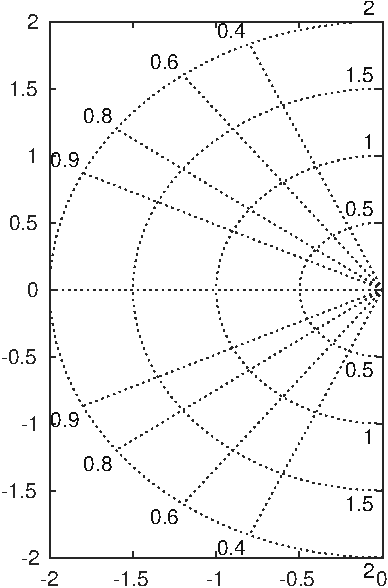
\includegraphics[height=0.34\textheight]{../../figures/sgrid-spring18-crop} \hspace*{3mm}
  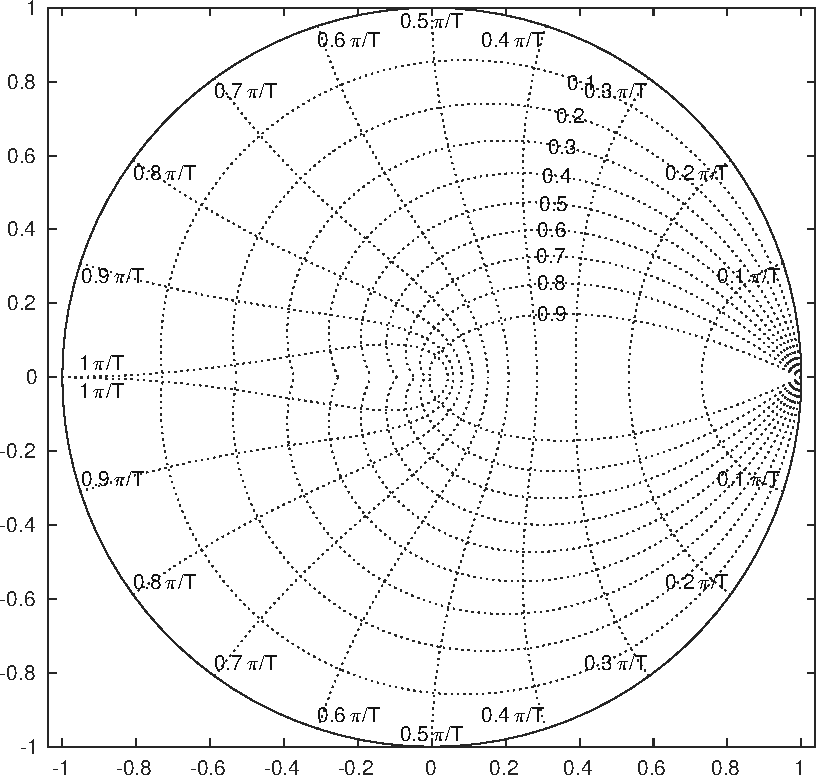
\includegraphics[height=0.34\textheight]{../../figures/zgrid-crop}\\
\end{center}
\noindent
\fbox{
\bmpl
{\bf Motivation for sampling period $h$ and calculations of discrete poles:}\\
\vspace*{40mm}
\emp}

\begin{figure}[!h]
  \begin{center}
    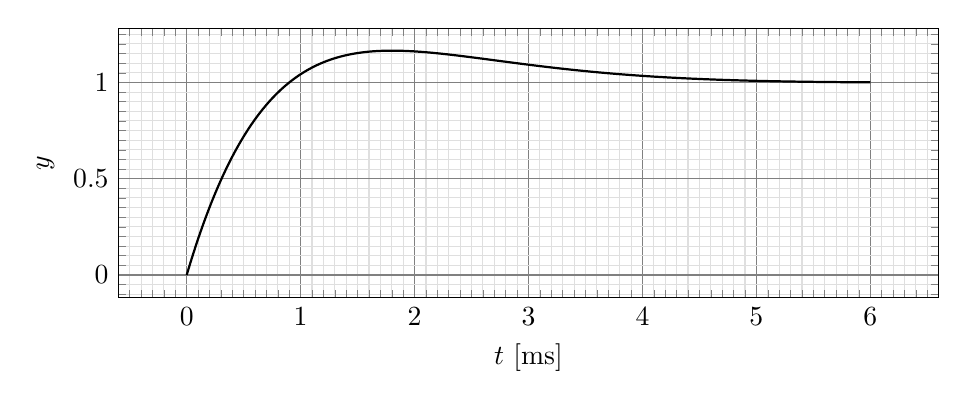
\begin{tikzpicture}
      
      \pgfmathsetmacro{\realpart}{1}
      \pgfmathsetmacro{\impart}{0.6}
      \pgfmathsetmacro{\wwn}{sqrt(pow(\realpart, 2) + pow(\impart, 2))}
      \pgfmathsetmacro{\zz}{\realpart/\wwn}
      \pgfmathsetmacro{\wwd}{\wwn*sqrt(1-pow(\zz,2))}
      \begin{axis} [
        width=12cm,
        height=5cm,
        xlabel = {$t$ [ms]},
        ylabel = {$y$},
        grid = both,
        minor tick num=9,
        minor grid style={gray!25},
        major grid style={black!50},
        ]
         \addplot+[thick, black, solid, no marks, domain=0:6, samples=400] { 1 + exp(-\zz*\wwn*x)/sqrt(1-pow(\zz,2))*sin(deg(\wwd*x) - acos(\zz)) };
      \end{axis}
    \end{tikzpicture}
    \caption{Step-response of desired closed-loop system (in continuous-time)}
    \label{fig:stepresponse}
  \end{center}
\end{figure}
\end{exercise}

%--------------------------------------------------------------------------------
% Exercise 2
%--------------------------------------------------------------------------------

\begin{exercise}
We now consider a model of the system in the unstable region ($a=-1$). Discretizing the continuous-time model in figure \ref{fig:openloopblock} gives the system shown in figure \ref{fig:openloopdt}.
\begin{figure}[!h]
\begin{center}
  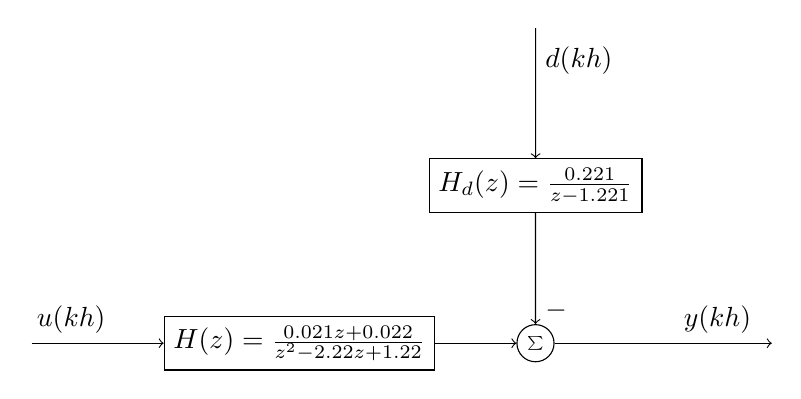
\begin{tikzpicture}[scale = 0.8, node distance=22mm, block/.style={rectangle, draw, minimum width=15mm}, sumnode/.style={circle, draw, inner sep=2pt}]
    
    \node[coordinate] (input) {};
     \node[block, right of=input, node distance=34mm] (plant) {$H(z) = \frac{0.021z + 0.022}{z^2 - 2.22z + 1.22}$};
     \node[sumnode, right of=plant, node distance=30mm] (sumdist) {\tiny $\sum$};
     \node[block, above of=sumdist, node distance=20mm] (distplant) {$H_d(z) = \frac{0.221}{z - 1.221}$};
     \node[coordinate, right of=sumdist, node distance=30mm] (output) {};
     \node[coordinate, above of=distplant, node distance=20mm] (dist) {};

     \draw[->] (input) -- node[above, pos=0.3] {$u(kh)$} (plant);
     \draw[->] (sumdist) -- node[above, near end] {$y(kh)$} (output);
     \draw[->] (plant) -- node[above, near end] {$$} (sumdist);
     \draw[->] (dist) -- node[right, near start] {$d(kh)$} (distplant);
     \draw[->] (distplant) -- node[right, very near end] {$-$} (sumdist);
   \end{tikzpicture}
   \caption{Open-loop discretized system.}
   \label{fig:openloopdt}
 \end{center}
\end{figure}

\abc Consider using the control law \[u(kh+h) = 0.2u(kh) + 10 \big( e(kh+h) - 0.9 e(kh) \big)\] where
\(e(kh) = y_{ref}(kh) - y(kh).\)
What type of controller is this (P, PI, PD, PID, Lead, Lag)? 

\noindent
\fbox{
  \bmpl
  {\bf Calculations:}\\
  \vspace*{30mm}
  \emp}
\abc
With the controller in (a), what is the closed-loop pulse-transfer function from the disturbance $d(kh)$ to the output $y(kh)$?

\noindent
\fbox{
  \bmpl
  {\bf Calculations:}\\
  \vspace*{56mm}
  \emp}

\abc
Figure \ref{fig:leadstep} shows the response of the output $y(kh)$ to a step in the disturbance $d(kh)$. The response goes to zero, meaning the steady-state error is zero. Why does the closed-loop system show this behaviour?

\noindent
\fbox{
  \bmpl
  {\bf Answer:}\\
  \vspace*{6mm}
  \emp}
\begin{figure}[!h]
  \begin{center}
    \begin{tikzpicture}
      \begin{axis} [
        width=12cm,
        height=6cm,
        xlabel = {$t$ [ms]},
        ylabel = {$y(kh)$},
        grid = both,
        minor tick num=9,
        minor grid style={gray!25},
        major grid style={black!50},
        ]
         \addplot+[thick, black, solid, const plot, no marks] table [x index = 0, y index =1, column sep=comma] {../../matlab/abs-lead-steps.dat};
      \end{axis}
    \end{tikzpicture}
    \caption{Response of the closed-loop system in Problem 2 to a step in the disturbance.}
    \label{fig:leadstep}
  \end{center}
\end{figure}


\abc
[Bonus question. Worth 4p] What is the sampling period $h$ and what is the Nyquist frequency for this sampled system?

\noindent
\fbox{
  \bmpl
  {\bf Answers:}\\
  \vspace*{20mm}
  \emp}



\end{exercise}


%\subsection*{Problem 3}
\begin{exercise}
The simple controller in Problem 2 gives a closed-loop system with three poles in 
\begin{equation}
 p_1 = 0.67, \quad p_2 = 0.77 + 0.28i, \quad p_3 = 0.77 - 0.28 i.
\label{eq:poles}
\end{equation}
The response of the system to a step in the disturbance which is shown in figure \ref{fig:leadstep} turned out to be unacceptable for the performance of the ABS system: It takes too long time to get back to the correct wheel velocity.  Moreover, the wheel velocity sensor is also quite noisy, so an antialiasing filter is needed, and the controller designen in Problem 2 beomes unstable when an antialiasing filter is present in the feedback path. Motivated by these issues, the 2-degrees-of-freedom controller in figure \ref{fig:2dof} is proposed. 
\begin{figure}[!h]
\begin{center}
  \begin{tikzpicture}[scale = 0.8, node distance=22mm, block/.style={rectangle, draw, minimum width=15mm}, sumnode/.style={circle, draw, inner sep=2pt}]
    
    \node[coordinate] (input) {};
     \node[block, right of=input, node distance=28mm] (Ff) {$F_f(z) = \frac{T(z)}{R(z)}$};
     \node[sumnode, right of=Ff, node distance=24mm] (sum) {\tiny $\sum$};
     \node[block, right of=sum, node distance=38mm] (plant) {$H(z) = \frac{0.021z + 0.022}{z^2 - 2.22z + 1.22}$};
     \node[sumnode, right of=plant, node distance=40mm] (sumdist) {\tiny $\sum$};
     \node[block, above of=sumdist, node distance=20mm] (distplant) {$H_d(z) = \frac{0.221}{z - 1.221}$};
     \node[block, below of=plant, node distance=24mm] (Fb) {$F_b(z) = \frac{S(z)}{R(z)}$};
     \node[block, below of=sumdist, node distance=24mm] (aa) {$z^{-2}$};
     \node[coordinate, right of=sumdist, node distance=35mm] (output) {};
     \node[coordinate, above of=distplant, node distance=20mm] (dist) {};

     \draw[->] (input) -- node[above, pos=0.3] {$y_{ref}(kh)$} (Ff);
     \draw[->] (Ff) -- node[above, pos=0.3] {$$} (sum);
     \draw[->] (sum) -- node[above, pos=0.5] {$u(kh)$} (plant);
     \draw[->] (sumdist) -- node[coordinate] (measure) {} node[above, near end] {$y(kh)$} (output);
     \node[sumnode, below of=measure, node distance=24mm] (sumnoise) {\tiny $\sum$};
     \draw[->] (plant) -- node[above, near end] {$$} (sumdist);
     \draw[->] (dist) -- node[right, near start] {$d(kh)$} (distplant);
     \draw[->] (measure) -- node[right, very near end] {} (sumnoise);
     \draw[->] (sumnoise) -- node[right, very near end] {} (aa);
     \draw[->] (aa) -- node[above, ] {$y_m(kh)$} (Fb);
     \draw[->] (Fb) -| node[right, very near end] {$-$} (sum);
     \draw[->] (distplant) -- node[right, very near end] {$-$} (sumdist);
     \draw[->] (sumnoise) ++(16mm,0) -- node[above,  near start] {$v(kh)$} (sumnoise);

   \end{tikzpicture}
   \caption{Two-degrees-of-freedom discrete controller. The signal $v(kh)$ represents the measurement noise.}
   \label{fig:2dof}
 \end{center}
\end{figure}

\abc
The Diophantine equation becomes
\begin{equation}
  A(z)z^2R(z) + B(z)S(z) = A_c(z)A_o(z)
  \label{eq:dioph}
\end{equation}
Write out the polynomials $A(z)$ and $B(z)$ in \eqref{eq:dioph}.

\noindent
\fbox{
  \bmpl
  {\bf Answers:}\\
  \vspace*{26mm}
  \emp}


\abc
What is the idea behind factorizing the right hand side of the Diophantine equation \eqref{eq:dioph} into the two polynomials \(A_c(z)A_o(z)\)?

\noindent
\fbox{
  \bmpl
  {\bf Answer:}\\
  \vspace*{46mm}
  \emp}


\abc
Determine the suitable order $n = \deg R$ of the controller 
\[ F_b(z) = \frac{S(z)}{R(z)}=\frac{s_0z^n + s_1z^{n-1} + \cdots + s_n}{z^n + r_1z^{n-1} + \cdots + r_n}\]
so that the parameters can be determined from the Diophantine equation \eqref{eq:dioph}.

\noindent
\fbox{
  \bmpl
  {\bf Calculations:}\\
  \vspace*{56mm}
  \emp}


\abc
[Bonus question. Worth 6p]
Assume that the sampled measured signal $y_m(kh)$ after the low-pass anti-aliasing filter has very good signal-to-noise-ratio (SNR), meaning $v(kh) \approx 0$ and we don't need to worry about the influence of measurement noise on the closed-loop system. Suggest closed-loop poles (roots of $A_c$) and observer poles (roots of $A_o$) such that 
\begin{itemize}
\item the response of the closed-loop system to the reference signal $y_{ref}(kh)$ is about twice as fast and better damped compared to the closed-loop system in Problem 2 with poles given in \eqref{eq:poles},    
\item the closed-loop system rejects the disturbance $d(kh)$ as fast as possible.
\end{itemize}
Plot the poles in \eqref{eq:poles}, together with your suggested poles in the z-plane below. Mark clearly which are the roots of $A_o(z)$ and which are the roots of $A_c(z)$.   
\begin{center}
  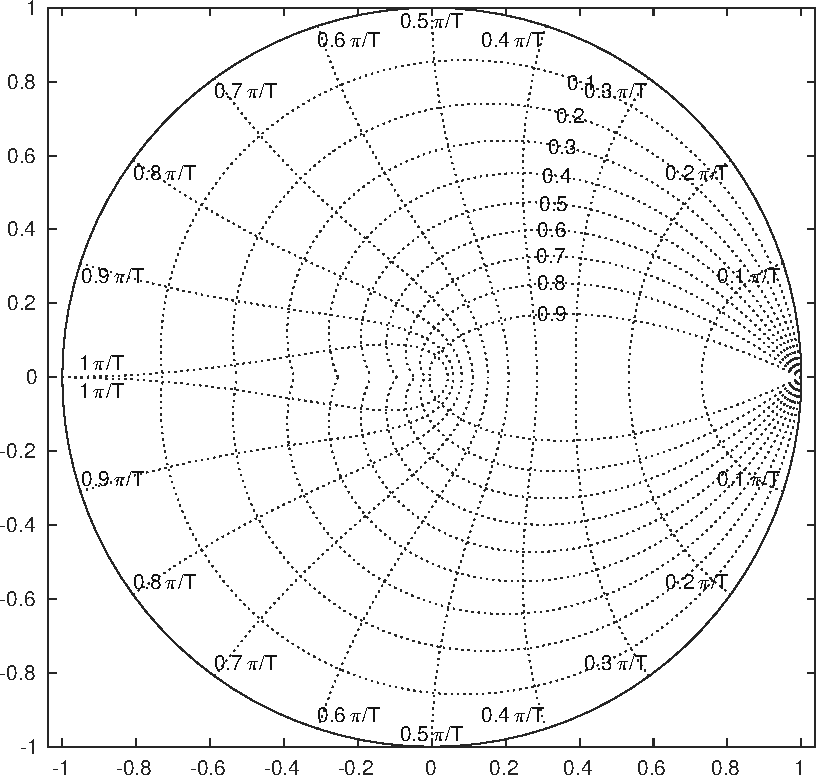
\includegraphics[width=0.6\linewidth]{../../figures/zgrid-crop}
\end{center}

\end{exercise}

\begin{exercise}
We want to identify a discrete-time model of a dynamical system
\begin{center}
  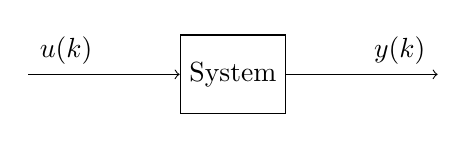
\begin{tikzpicture}[node distance=2.6cm, block/.style={rectangle, draw, minimum height=10mm, minimum width=12mm}, sumnode/.style={circle, draw, inner sep=1pt}]
  \node[coordinate] (input) {};
  \node[block,  right of=input] (ssys) {System};
  \node[coordinate, right of=ssys] (output) {};
  \draw[->] (input) -- node[above, near start] {$u(k)$} (ssys);
  \draw[->] (ssys) -- node[above, near end] {$y(k)$} (output);
\end{tikzpicture}
\end{center}
based on the collected input-output data $\{(u_i, y_i)\}, \; i=1,2,\ldots, N$, where we assume the model
\begin{equation*}
  \shift^2 y(k) + a_1\shift y(k) + a_2 y(k) = b_0\shift u(k) + b_1 u(k) + \shift^2 e(k),
%  \label{eq:demodel}
\end{equation*}
where $e(k)$ is a white noise sequence. 
\abc Write out the one-step ahead predictor $\hat{y}(k+1)$ for the model

\noindent
\fbox{
  \bmpl
  {\bf Answer:}\\
  \vspace*{16mm}
  \emp}

\abc Which of the below equations (1--4) is correct for determining the least squares estimate of the model parameter? Circle your answer!

\begin{enumerate}
  \item
    \begin{displaymath}
      \bbm -y(2) & -y(1) & u(3) & u(2)\\
      -y(3) & -y(2) & u(4) & u(3)\\
      \vdots & \vdots & \vdots & \vdots\\
      -y(N-1) & -y(N-2) & u(N) & u(N-1)\ebm \bbm a_1\\a_2\\b_0\\b_1\ebm = \bbm y(3)\\y(4)\\\vdots\\y(N)\ebm
    \end{displaymath}
  \item
    \begin{displaymath}
      \bbm -y(2) & -y(1) & u(2) & u(1)\\
      -y(3) & -y(2) & u(3) & u(2)\\
      \vdots & \vdots & \vdots & \vdots\\
      -y(N-1) & -y(N-2) & u(N-1) & u(N-2)\ebm \bbm a_1\\a_2\\b_0\\b_1\ebm = \bbm y(3)\\y(4)\\\vdots\\y(N)\ebm
    \end{displaymath}
  \item
    \begin{displaymath}
      \bbm -y(3) & -y(2) & u(2) & u(1)\\
      -y(3) & -y(2) & u(3) & u(2)\\
      \vdots & \vdots & \vdots & \vdots\\
      -y(N-1) & -y(N-2) & u(N-1) & u(N-2)\ebm \bbm a_1\\a_2\\b_0\\b_1\ebm = \bbm y(4)\\y(5)\\\vdots\\y(N)\ebm
    \end{displaymath}
  \item
    \begin{displaymath}
      \bbm -y(2) & -y(1) & u(2) & u(1)\\
      -y(3) & -y(2) & u(3) & u(2)\\
      \vdots & \vdots & \vdots & \vdots\\
      -y(N-1) & -y(N-2) & u(N-1) & u(N-2)\ebm \bbm a_1\\a_2\\b_0\\b_1\ebm = \bbm y(4)\\y(5)\\\vdots\\y(N)\ebm
    \end{displaymath}
  \end{enumerate}
\end{exercise}

%\cleardoublepage
%\end{document} 

\section*{Solutions}

\setcounter{exerctr}{0} 

\pgfmathsetmacro{\omegan}{sqrt(1+pow(0.6, 2))}
\pgfmathsetmacro{\omeganhertz}{\omegan * 1000/2/pi}
\pgfmathsetmacro{\hh}{0.2}
\pgfmathsetmacro{\pdreal}{exp(-\hh)*cos(deg(0.6*\hh))}
\pgfmathsetmacro{\pdim}{exp(-\hh)*sin(deg(0.6*\hh))}
\begin{exercise}
\abc The natural frequency $\omega_n$ of a pair of complex-conjugated poles is the distance to the origin, which is 
\[ \omega_n = \sqrt{1 + 0.6^2} = \unit{\omegan}{\rad\per\milli\second}. \]
In Hz this becomes
\[ \omegan \frac{1000}{2\pi} = \unit{\omeganhertz}{\hertz}. \]

\abc
The textbook in chapter 2.9 ``Selection of sampling rate'' suggests a rule-of-thumb for complex-valued poles \[\omega_n h \approx 0.2 - 0.6.\] So any value in this range would be an acceptable choice. It would also be acceptable to look at the step-response and use the rule-of-thumb that \[\frac{T_r}{h} \approx 4 - 10,\] where $T_r$ is the rise time of the step-response. Here, $\omega_n = \omegan$, so I choose $h = 0.2$, which gives the discrete-time poles \[ p_{1,2} = \mexp{(-1 \pm 0.6i)h} = \mexp{-0.2}\big(\cos(0.12)  \pm i\sin(0.12)\big) = \pdreal \pm i \pdim. \]
\begin{center}
  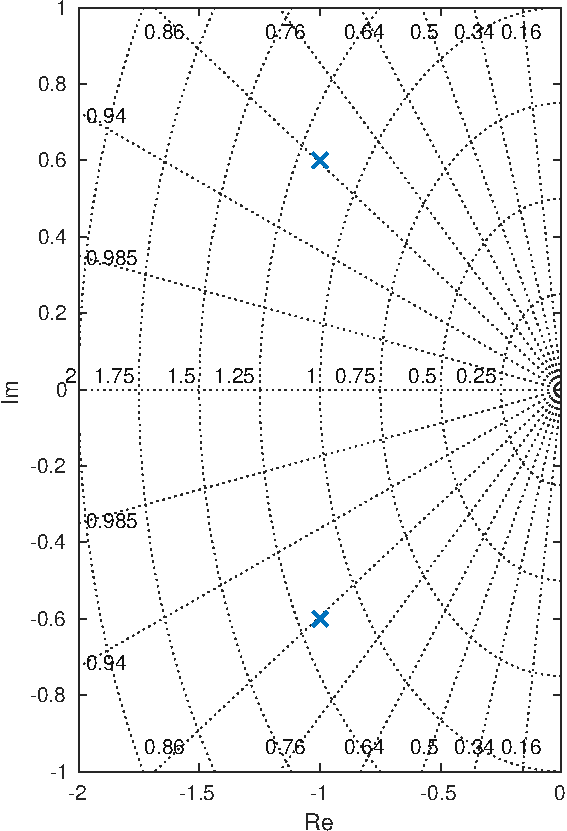
\includegraphics[width=0.36\linewidth]{abs-desired0-cont-poles-crop} \hspace*{2mm}
  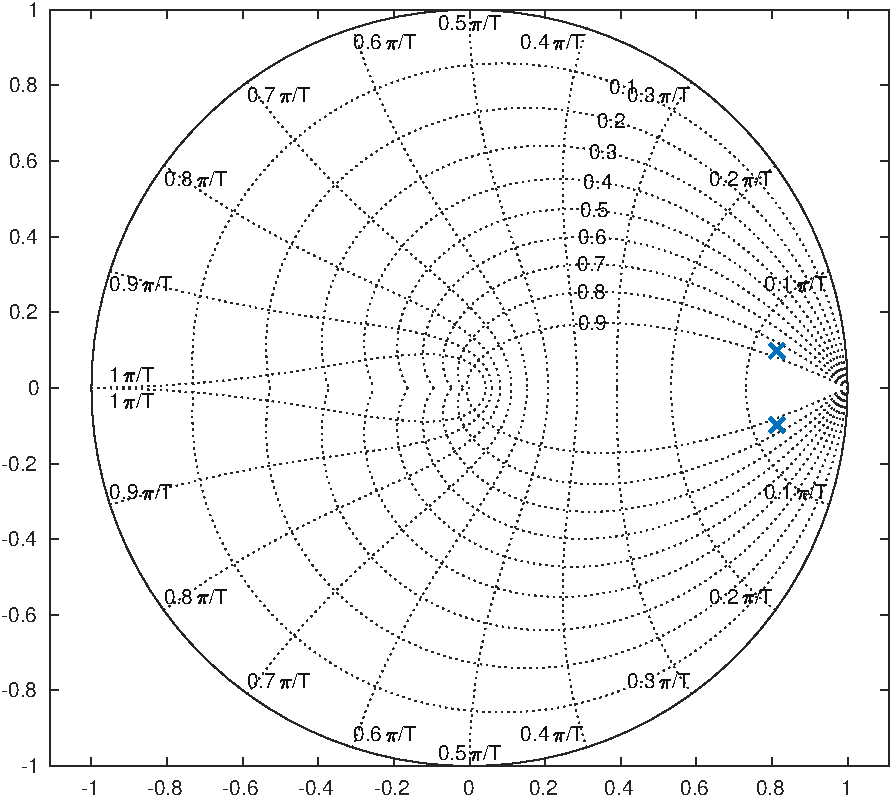
\includegraphics[width=0.58\linewidth]{abs-desired0-poles-crop}
\end{center}
\end{exercise}

\begin{exercise}
\abc The pulse-transfer operator for the controller is \[F(\shift) = 10 \frac{\shift - 0.9}{\shift - 0.2},\] which has a zero in 0.9 and a pole in 0.2. A first-order system with the zero closer to 1 than the pole. That is clearly a \textbf{lead controller}.

\abc The controller is \[ F(z) = 10\frac{z-0.9}{z-0.2}.\] Using Mason's rule we get the transfer function from the disturbance $d(kh)$ to the output $y(kh)$ 
\begin{equation*}
  \begin{aligned}
    G_{cd}(z) &= \frac{H_d(z)}{1 + F(z)H(z)} = \frac{\frac{0.221}{z-1.221}}{ 1 + 10\frac{z-0.9}{z-0.2}\cdot\frac{0.021z + 0.022}{(z-1)(z-1.221)}}\\
    &= \frac{0.221(z-1)(z-0.2)}{(z-1)(z-1.1221)(z-0.2) + 10(z-0.9)}
  \end{aligned}
\end{equation*}

\abc The constant disturbance is eliminated because the loop gain contains an integration. We can also show this using the final-value theorem
\begin{equation*}
  \begin{aligned}
    \lim_{k\to\infty} y(kh) &= \lim_{z\to 1} (z-1) Y(z) =\lim_{z\to 1} (z-1) G_{cd}(z) \frac{z}{z-1}\\
    &= G_{cd}(1) = 0.
  \end{aligned}
\end{equation*}

\abc There are basically two ways to figure out the sampling period. The easiest is just to look carefully at the time-plot in figure \ref{fig:leadstep}. There are clearly 5 samples for each millisecond, so $h=\unit{0.2}{\milli\second}$. It can also be noted by the fact that the continuous-time model has a pole in $s=a=1$, which in the discrete-time model shows up in $z=1.221 = \mexp{ah} = \mexp{h}$ so $h = \ln 1.1221 = 0.2$. The Nyquist frequency is given by
\pgfmathsetmacro{\omegaN}{pi/0.2}
\[ \omega_N = \frac{\pi}{h} = \unit{\omegaN}{\radian\per\milli\second}.\]
\end{exercise}

\begin{exercise}
\abc $B(z)$ is the numerator of the plant model, so $B(z) = 0.021z + 0.022$. $A(z)$ is the denominator $A(z) = z^2 - 2.22z + 1.22$.
\abc The idea behind factorizing the desired characteristic polynomial is that we can use one factor $A_c(z)$ to determine a desired response of the closed-loop system to the reference signal, and we can use $A_o(z)$ (the observer polynomial) to determine a desired trade-off between disturbance rejection (fast observer poles) and attenuation of measurement noise (slow observer poles). By letting $T(z) = t_0A_o(z)$, the observer poles are cancelled in the closed-loop pulse transfer function from $y_{ref}$ to $y$.
\abc The number of unknowns in the controller is $2n+1$, and the number of equations obtained from setting the coefficients of the left- and right hand side equal in the Diophantine equation is the same as the degree of the polynomials. This degree is $n + \deg A + 2$. We get
\[ 2n+1 = n + \deg A + 2 \quad \Rightarrow \quad n = \deg A + 1 = 3.\]
\abc The degree of the left hand side of the Diophantine equation will be $2+2+3=7$, so we need to specify 7 poles. Since $F_f(z) = \frac{T(z)}{R(z)} = \frac{t_0A_o(z)}{R(z)}$, and the system $F_f(z)$ must be causal, we have that $\deg A_o \le \deg R$ so the observer polynomial should be of degree 3 (or less). Since we had good SNR in the feedback signal, and want to have good disturbance rejection, we choose the fastest observer poles possible, which mean in the origin
\[ A_o(z) = z^3.\]
This leaves four poles to be placed for $A_c(z)$. Plotting the three closed-loop poles for the system in Problem 2 
\begin{center}
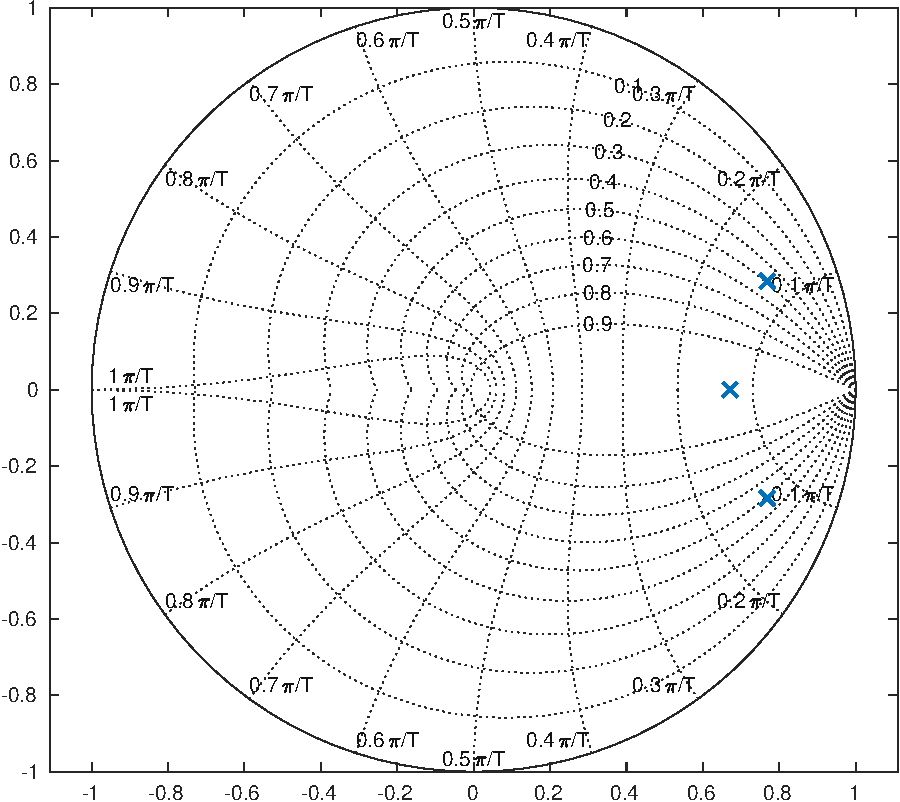
\includegraphics[width=0.5\linewidth]{../../matlab/abs-lead-poles-crop}
\end{center}
we see that the speed (distance from 1) is about 1.3 and the damping ratio about 0.5 for the two complex-conjugated poles. Improving the speed (twice as fast) and the damping gives the following suggested poles. Green crosses are observer poles, red crosses the suggested roots of $A_c(z)$.
\begin{center}
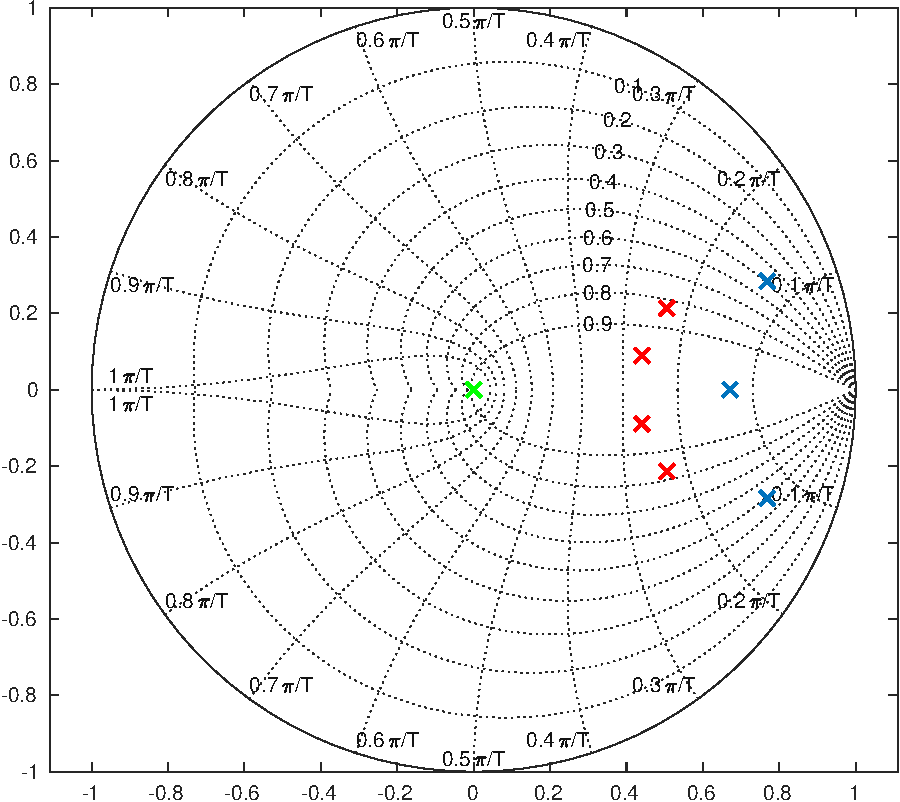
\includegraphics[width=0.5\linewidth]{../../matlab/abs-desired-poles-crop}
\end{center}

Completing the design (not asked for) will give the following controller
\begin{align*}
  F_b(z) &= \frac{29.32 z^3 - 27.21z^2}{z^3 + 0.330z^2 + 0.905z + 0.510}\\
  F_f(z) &= \frac{2.105z^3}{z^3 + 0.330z^2 + 0.905z + 0.510}
\end{align*}
with the following response to a step disturbance in $d(kh)$
  \begin{center}
    \begin{tikzpicture}
      \begin{axis} [
        width=12cm,
        height=6cm,
        xlabel = {$t$ [ms]},
        ylabel = {$y(kh)$},
        grid = both,
        minor tick num=9,
        minor grid style={gray!25},
        major grid style={black!50},
        ]
         \addplot+[thick, black, solid, const plot, no marks] table [x index = 0, y index =1, column sep=comma] {../../matlab/abs-rst-steps.dat};
      \end{axis}
    \end{tikzpicture}
  \end{center}

\end{exercise}

\begin{exercise}
\abc With the model
\begin{equation*}
  \begin{aligned}
  \shift^2 y(k) + a_1\shift y(k) + a_2 y(k) &= b_0\shift u(k) + b_1 u(k) + \shift^2 e(k),\\[2mm]
  &\Updownarrow\\[2mm]
  y(k+2) &= -a_1y(k+1) - a_2y(k) + b_0u(k+1) + b_1u(k) + e(k+2),
%  \label{eq:demodel}
\end{aligned}
\end{equation*}
the one-step ahead predictor becomes
\[ \hat{y}(k+1) = -a_1y(k) - a_2y(k-1) + b_0u(k) + b_1u(k-1).\]

\abc The correct equation is 2.
    \begin{displaymath}
      \bbm -y(2) & -y(1) & u(2) & u(1)\\
      -y(3) & -y(2) & u(3) & u(2)\\
      \vdots & \vdots & \vdots & \vdots\\
      -y(N-1) & -y(N-2) & u(N-1) & u(N-2)\ebm \bbm a_1\\a_2\\b_0\\b_1\ebm = \bbm y(3)\\y(4)\\\vdots\\y(N)\ebm
    \end{displaymath}


\end{exercise}


\end{document}
